\documentclass[DM,toc]{lsstdoc}
\usepackage{geometry}
\usepackage{longtable,booktabs,graphicx}
\usepackage{enumitem}
\usepackage{arydshln}
% lsstdoc documentation: https://lsst-texmf.lsst.io/lsstdoc.html

% Generated by Makefile
\input{meta}

% Package imports go here.

% Local commands go here.

% If you want glossaries, uncomment:
% \input{aglossary.tex}
% \makeglossaries

\title{Characterization Metric Report: Science Pipelines Version 29.0}
% \setDocSubtitle{Optional subtitle}

\author{%
Jeff Carlin
}

\setDocRef{DMTR-461}
\setDocUpstreamLocation{\url{https://github.com/lsst-dm/DMTR-461}}
\date{\vcsDate}
% \setDocCurator{The Curator of this Document}

\setDocAbstract{%
This brief report describes measurements of data quality metrics that were carried out for release v29.0.0 of the LSST Science Pipelines. The report for the previous version can be found in \citedsp{DMTR-451}.
}

% Revision history.
% Order: oldest first.
% Fields: VERSION, DATE, DESCRIPTION, OWNER NAME.
% See LPM-51 for version number policy.
\setDocChangeRecord{%
  \addtohist{1}{2025-05-28}{Unreleased.}{Jeff Carlin}
}

\begin{document}

\maketitle

In this report, we characterize the performance of the Rubin Observatory Science Pipelines Version 29.0.0. We illustrate the performance via metrics that are measured on the HSC-RC2 dataset. RC2 consists of 3 tracts of data taken from the HSC-SSP survey, and selected to provide a means of testing various ``pathological'' cases (e.g., difficult astrometric solutions, extremely good seeing that does not provide a well-sampled PSF, difficult fields for deblending, and large galaxies, among others). These three tracts each contain between 112--149 visits split between the HSC-G, HSC-R, HSC-I, HSC-Z, and HSC-Y (\emph{grizy}) filters.

Between w\_2024\_42 (the source for pipelines version 28) and w\_2025\_09 (v29 source), most major changes in the science pipelines have been in supporting packages and not to algorithms that dramatically affected the Data Release processing metrics. As of v28, the streak-detection algorithm introduced in v21 operates on image differences instead of direct images. This algorithm masks pixels affected by streaks (e.g., satellites or other trailed sources of non-astrophysical origin). Previously, streaks were only removed during coaddition.

Additional new features in this release include:
\begin{itemize}
    \item Object now contains only primary objects (i.e., "detect\_isPrimary == True"), and non-primaries are saved in a separate table.
    \item Illumination correction frames (DM-22491)
    \item ArrowAstropy is default table return now?
    \item Calibrate/characterize completely changed?
    \item New code to deal with new image defects (e.g., vampire pixels, ITL edge bleeds, etc.)?
    \item Now using the Monster as default refcat
    \item 
    \item The use of ``compensated tophats'' to measure fluxes used in photometric calibration \href{https://rubinobs.atlassian.net/browse/DM-38632}{(DM-38632)}, which are applied in CalibrateImageTa
sk \href{https://rubinobs.atlassian.net/browse/DM-44908}{(DM-44908)}.
    \item The default signal-to-noise cut for PSF star selection was increased from 20 to 50 \href{https://rubinobs.atlassian.net/browse/DM-44130}{(DM-44130)}.
    \item Interpolation of bad pixels is now done via a Gaussian Process algorithm \href{https://rubinobs.atlassian.net/browse/DM-44305}{(DM-44305)}.
\end{itemize}

Photometry and astrometry metrics reported here were calculated using the \href{https://github.com/lsst/analysis_tools}{analysis\_tools} package, which is part of the standard pipeline distribution. The \texttt{analysis\_tools} package builds on and supersedes \href{https://github.com/lsst/faro}{faro} (\citeds{DMTN-211}), which has been used for the past few years. The calculation of most metrics reported in this Report is unchanged between the two packages, though minor differences in how selection criteria are applied, or how catalog matching is done, between \texttt{analysis\_tools} and \texttt{faro} could result in small differences in the resulting metrics. We are actively working on a revised definition of the residual ellipticity correlation metrics TE1 and TE2, to be implemented in \texttt{analysis\_tools}. Because this work is still in progress, the ellipticity metrics are not reported here.

The metric calculation pipelines from \texttt{analysis\_tools} were run on the three RC2 tracts to derive the photometry and astrometry metrics
% , and \texttt{faro} to calculate the shape metrics
that are reported here. We exclude the two astrometry metrics (AM3 and AF3) that concern residuals on 200-arcminute scales, since the individual tracts of RC2 do not span large enough spatial scales to enable these measurements.

For comparison, we provide the \SRD required ``design'' value of each Key Performance Metric (KPM) as defined in the Science Requirements Document \citedsp{LPM-17}. For the ellipticity correlation metrics, there are specifications only for \emph{r} and \emph{i} bands. The \emph{ugzy}-band measurements are of interest primarily for historical tracking.

Some KPMs (e.g., PF1, AF1, AF2) involve thresholds that are different for ``design'', ``minimum'', and ``stretch'' specifications. Metrics in this report are all compared to the ``design'' thresholds. The assessment of these KPMs would be different if evaluated against different thresholds.

\textbf{DP1 LSSTComCam On-sky Data:} Version~29 of the Science Pipelines was used for processing of the Data Preview 1 (DP1) data, which derived from on-sky commissioning conducted with LSSTComCam, the commissioning camera (ADD DP1 PAPER REF AND SITCOMTN-149 REF?). Here we report the photometry and astrometry metrics as measured on tract 5063, one of the tracts that overlaps the ECDFS field of view in DP1. The metrics are presented in the tables and figures of this report for comparison to the same metrics measured on HSC-RC2 data. However, these should not be directly compared, as the LSSTComCam data were commissioning data taken with a newly-installed camera before the system had been optimized. Thus these v29 metrics based on LSSTComCam DP1 data should be taken as a starting point for future comparisons with on-sky LSST data, which are likely to significantly improve upon the performance shown here.

\begin{figure}[!t]
  \centering
  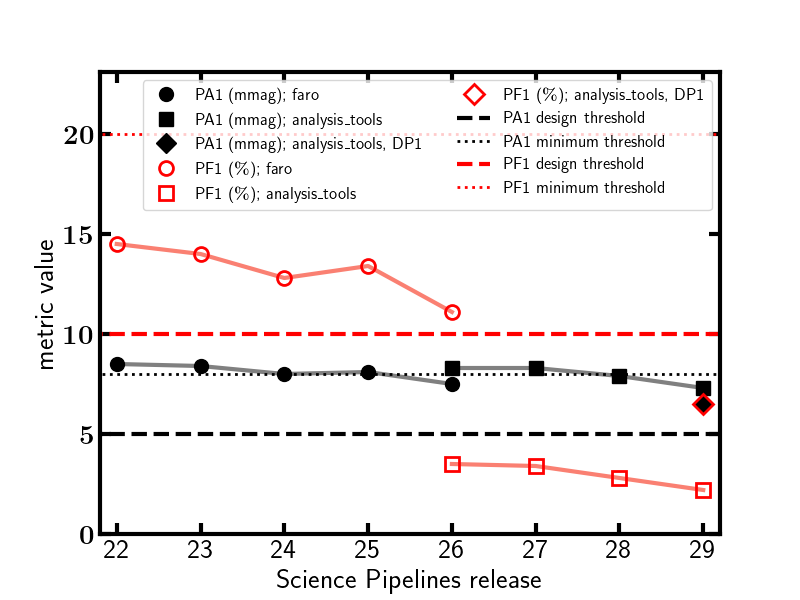
\includegraphics[width=0.6\textwidth, trim=0.0in 0.0in 0.0in 0.0in, clip]{figures/photom_metrics_v29_with_thresholds.png}
  \caption{Photometry metrics PA1 (photometric repeatability) and PF1 (percentage of measurements exceeding the outlier threshold) measured in the $r$-band. The figure shows the values of these metrics as measured with \texttt{faro} in versions 22-26 of the LSST Science Pipelines as circles, compared against the SRD requirements (for both the ``design'' and ``minimum'' thresholds). The measurements from \texttt{analysis\_tools} in versions 26-28 of the Science Pipelines are shown as squares. The measured values of both metrics show only minor changes between the two most recent releases (v27 and v28). The algorithm to calculate PA1 is unchanged between \texttt{faro} and \texttt{analysis\_tools} (though because of differences in software architecture, it is expected that we would see minor differences in their outputs), and the metric differs by only a small offset between the two versions calculated in v26. However, while porting the PF1 metric to \texttt{analysis\_tools}, we discovered an error in the method of calculation (see the text for details). Fixing this error reduced the value of PF1 significantly.}
  \label{fig:phot_metrics}
\end{figure}

\section{Summary of performance metrics}

As noted previously, we now report metrics calculated by the \texttt{analysis\_tools} package, which improves upon the \texttt{faro} tools we had been previously using for calculation of data quality metrics. The plots in this Report include metrics from both \texttt{analysis\_tools} and \texttt{faro} for historical continuity, but future data processing campaigns will not run the \texttt{faro} tasks. One significant change is evident when comparing the outputs of the two frameworks on the v26 dataset: in Figure~\ref{fig:phot_metrics}, PF1 is much smaller as measured by \texttt{analysis\_tools} than from \texttt{faro}. This is expected, as we discovered an error in the calculation that was fixed when porting the PF1 metric from \texttt{faro} to \texttt{analysis\_tools} (see \href{https://rubinobs.atlassian.net/browse/DM-39332}{Jira ticket DM-39332} for details). The previous version had been calculating the outlier fraction relative to a fixed value of 15 mmag, while the metric is intended to be the fraction of outliers \textit{more than 15 mmag from the median} photometric repeatability. The changes on DM-39332 have brought the PF1 metric's calculation in line with the description in the DMSR, resulting in a value that is well beneath the design threshold for PF1.

As noted in the previous section, most of the changes between versions 27 and 28 of the pipelines are minor, so the data quality metrics should also be similar. Indeed, the photometry metrics (Section~\ref{photometric-performance}) show slight improvements, and the astrometry metrics (Section~\ref{astrometric-performance}) are virtually unchanged.
The ellipticity correlation metrics (Section~\ref{ellipticity-correlations}) show only a small difference between Release 27 and 28 for TE1 (median ellipticity residual correlations at 1 arcminute scales) and TE2 (5-arcminute scales).

\section{Photometric Performance}\label{photometric-performance}
% NOTE: In v28, add the calib flux repeatability!

These photometric performance metrics are defined in LSS-REQ-0093 (\citeds{LSE-29}) and Table 14 of \citeds{LPM-17}. Values in this table represent the mean of the results reported by \texttt{analysis\_tools} for the three tracts in RC2.

Any entries left blank are those for which we do not have data in the given filter for that dataset.

\begin{longtable}[]{@{}lllllll@{}}
\toprule
\begin{minipage}[b]{0.12\columnwidth}\raggedright\strut
Metric\strut
\end{minipage} & \begin{minipage}[b]{0.06\columnwidth}\raggedright\strut
Unit\strut
\end{minipage} & \begin{minipage}[b]{0.14\columnwidth}\raggedright\strut
SRD Requirement -- Design\strut
\end{minipage} & \begin{minipage}[b]{0.12\columnwidth}\raggedright\strut
Release 28 Value (RC2) \strut
\end{minipage} & \begin{minipage}[b]{0.12\columnwidth}\raggedright\strut
Release 29 Value (RC2) \strut
\end{minipage} & \begin{minipage}[b]{0.12\columnwidth}\raggedright\strut
Release dp1\_v29 Value (ComCam) \strut
\end{minipage} & \begin{minipage}[b]{0.17\columnwidth}\raggedright\strut
Comments\strut
\end{minipage}\tabularnewline
\midrule
\endhead
\begin{minipage}[t]{0.12\columnwidth}\raggedright\strut
PA1: \emph{u}\strut
\end{minipage} & \begin{minipage}[t]{0.06\columnwidth}\raggedright\strut
mmag\strut
\end{minipage} & \begin{minipage}[t]{0.14\columnwidth}\raggedright\strut
\(\leq 7.5\)\strut
\end{minipage} & \begin{minipage}[t]{0.12\columnwidth}\raggedright\strut
nan \strut
\end{minipage} & \begin{minipage}[t]{0.12\columnwidth}\raggedright\strut
nan \strut
\end{minipage} & \begin{minipage}[t]{0.12\columnwidth}\raggedright\strut
7.1 \strut
\end{minipage} & \begin{minipage}[t]{0.17\columnwidth}\raggedright\strut

\end{minipage}\tabularnewline
\begin{minipage}[t]{0.12\columnwidth}\raggedright\strut
PA1: \emph{g}\strut
\end{minipage} & \begin{minipage}[t]{0.06\columnwidth}\raggedright\strut
mmag\strut
\end{minipage} & \begin{minipage}[t]{0.14\columnwidth}\raggedright\strut
\(\leq 5.0\)\strut
\end{minipage} & \begin{minipage}[t]{0.12\columnwidth}\raggedright\strut
7.8 \strut
\end{minipage} & \begin{minipage}[t]{0.12\columnwidth}\raggedright\strut
7.1 \strut
\end{minipage} & \begin{minipage}[t]{0.12\columnwidth}\raggedright\strut
8.9 \strut
\end{minipage} & \begin{minipage}[t]{0.17\columnwidth}\raggedright\strut

\end{minipage}\tabularnewline
\begin{minipage}[t]{0.12\columnwidth}\raggedright\strut
PA1: \emph{r}\strut
\end{minipage} & \begin{minipage}[t]{0.06\columnwidth}\raggedright\strut
mmag\strut
\end{minipage} & \begin{minipage}[t]{0.14\columnwidth}\raggedright\strut
\(\leq 5.0\)\strut
\end{minipage} & \begin{minipage}[t]{0.12\columnwidth}\raggedright\strut
7.9 \strut
\end{minipage} & \begin{minipage}[t]{0.12\columnwidth}\raggedright\strut
7.3 \strut
\end{minipage} & \begin{minipage}[t]{0.12\columnwidth}\raggedright\strut
6.5 \strut
\end{minipage} & \begin{minipage}[t]{0.17\columnwidth}\raggedright\strut

\end{minipage}\tabularnewline
\begin{minipage}[t]{0.12\columnwidth}\raggedright\strut
PA1: \emph{i}\strut
\end{minipage} & \begin{minipage}[t]{0.06\columnwidth}\raggedright\strut
mmag\strut
\end{minipage} & \begin{minipage}[t]{0.14\columnwidth}\raggedright\strut
\(\leq 5.0\)\strut
\end{minipage} & \begin{minipage}[t]{0.12\columnwidth}\raggedright\strut
8.1 \strut
\end{minipage} & \begin{minipage}[t]{0.12\columnwidth}\raggedright\strut
7.5 \strut
\end{minipage} & \begin{minipage}[t]{0.12\columnwidth}\raggedright\strut
6.2 \strut
\end{minipage} & \begin{minipage}[t]{0.17\columnwidth}\raggedright\strut

\end{minipage}\tabularnewline
\begin{minipage}[t]{0.12\columnwidth}\raggedright\strut
PA1: \emph{z}\strut
\end{minipage} & \begin{minipage}[t]{0.06\columnwidth}\raggedright\strut
mmag\strut
\end{minipage} & \begin{minipage}[t]{0.14\columnwidth}\raggedright\strut
\(\leq 7.5\)\strut
\end{minipage} & \begin{minipage}[t]{0.12\columnwidth}\raggedright\strut
6.5 \strut
\end{minipage} & \begin{minipage}[t]{0.12\columnwidth}\raggedright\strut
6.1 \strut
\end{minipage} & \begin{minipage}[t]{0.12\columnwidth}\raggedright\strut
7.3 \strut
\end{minipage} & \begin{minipage}[t]{0.17\columnwidth}\raggedright\strut
\end{minipage}\tabularnewline
\begin{minipage}[t]{0.12\columnwidth}\raggedright\strut
PA1: \emph{y}\strut
\end{minipage} & \begin{minipage}[t]{0.06\columnwidth}\raggedright\strut
mmag\strut
\end{minipage} & \begin{minipage}[t]{0.14\columnwidth}\raggedright\strut
\(\leq 7.5\)\strut
\end{minipage} & \begin{minipage}[t]{0.12\columnwidth}\raggedright\strut
6.9 \strut
\end{minipage} & \begin{minipage}[t]{0.12\columnwidth}\raggedright\strut
6.3 \strut
\end{minipage} & \begin{minipage}[t]{0.12\columnwidth}\raggedright\strut
6.0 \strut
\end{minipage} & \begin{minipage}[t]{0.17\columnwidth}\raggedright\strut
\end{minipage}\tabularnewline
\begin{minipage}[t]{0.12\columnwidth}\raggedright\strut
PF1: \emph{u}\strut
\end{minipage} & \begin{minipage}[t]{0.06\columnwidth}\raggedright\strut
\%\strut
\end{minipage} & \begin{minipage}[t]{0.14\columnwidth}\raggedright\strut
\(\leq 10.0\)\strut
\end{minipage} & \begin{minipage}[t]{0.12\columnwidth}\raggedright\strut
nan \strut
\end{minipage} & \begin{minipage}[t]{0.12\columnwidth}\raggedright\strut
nan \strut
\end{minipage} & \begin{minipage}[t]{0.12\columnwidth}\raggedright\strut
2.2 \strut
\end{minipage} & \begin{minipage}[t]{0.17\columnwidth}\raggedright\strut
\end{minipage}\tabularnewline
\begin{minipage}[t]{0.12\columnwidth}\raggedright\strut
PF1: \emph{g}\strut
\end{minipage} & \begin{minipage}[t]{0.06\columnwidth}\raggedright\strut
\%\strut
\end{minipage} & \begin{minipage}[t]{0.14\columnwidth}\raggedright\strut
\(\leq 10.0\)\strut
\end{minipage} & \begin{minipage}[t]{0.12\columnwidth}\raggedright\strut
4.2 \strut
\end{minipage} & \begin{minipage}[t]{0.12\columnwidth}\raggedright\strut
2.7 \strut
\end{minipage} & \begin{minipage}[t]{0.12\columnwidth}\raggedright\strut
3.4 \strut
\end{minipage} & \begin{minipage}[t]{0.17\columnwidth}\raggedright\strut
\end{minipage}\tabularnewline
\begin{minipage}[t]{0.12\columnwidth}\raggedright\strut
PF1: \emph{r}\strut
\end{minipage} & \begin{minipage}[t]{0.06\columnwidth}\raggedright\strut
\%\strut
\end{minipage} & \begin{minipage}[t]{0.14\columnwidth}\raggedright\strut
\(\leq 10.0\)\strut
\end{minipage} & \begin{minipage}[t]{0.12\columnwidth}\raggedright\strut
2.8 \strut
\end{minipage} & \begin{minipage}[t]{0.12\columnwidth}\raggedright\strut
2.2 \strut
\end{minipage} & \begin{minipage}[t]{0.12\columnwidth}\raggedright\strut
6.5 \strut
\end{minipage} & \begin{minipage}[t]{0.17\columnwidth}\raggedright\strut
\end{minipage}\tabularnewline
\begin{minipage}[t]{0.12\columnwidth}\raggedright\strut
PF1: \emph{i}\strut
\end{minipage} & \begin{minipage}[t]{0.06\columnwidth}\raggedright\strut
\%\strut
\end{minipage} & \begin{minipage}[t]{0.14\columnwidth}\raggedright\strut
\(\leq 10.0\)\strut
\end{minipage} & \begin{minipage}[t]{0.12\columnwidth}\raggedright\strut
1.9 \strut
\end{minipage} & \begin{minipage}[t]{0.12\columnwidth}\raggedright\strut
1.6 \strut
\end{minipage} & \begin{minipage}[t]{0.12\columnwidth}\raggedright\strut
0.2 \strut
\end{minipage} & \begin{minipage}[t]{0.17\columnwidth}\raggedright\strut
\end{minipage}\tabularnewline
\begin{minipage}[t]{0.12\columnwidth}\raggedright\strut
PF1: \emph{z}\strut
\end{minipage} & \begin{minipage}[t]{0.06\columnwidth}\raggedright\strut
\%\strut
\end{minipage} & \begin{minipage}[t]{0.14\columnwidth}\raggedright\strut
\(\leq 10.0\)\strut
\end{minipage} & \begin{minipage}[t]{0.12\columnwidth}\raggedright\strut
1.1 \strut
\end{minipage} & \begin{minipage}[t]{0.12\columnwidth}\raggedright\strut
0.9 \strut
\end{minipage} & \begin{minipage}[t]{0.12\columnwidth}\raggedright\strut
1.0 \strut
\end{minipage} & \begin{minipage}[t]{0.17\columnwidth}\raggedright\strut
\end{minipage}\tabularnewline
\begin{minipage}[t]{0.12\columnwidth}\raggedright\strut
PF1: \emph{y}\strut
\end{minipage} & \begin{minipage}[t]{0.06\columnwidth}\raggedright\strut
\%\strut
\end{minipage} & \begin{minipage}[t]{0.14\columnwidth}\raggedright\strut
\(\leq 10.0\)\strut
\end{minipage} & \begin{minipage}[t]{0.12\columnwidth}\raggedright\strut
1.7 \strut
\end{minipage} & \begin{minipage}[t]{0.12\columnwidth}\raggedright\strut
1.1 \strut
\end{minipage} & \begin{minipage}[t]{0.12\columnwidth}\raggedright\strut
0.0 \strut
\end{minipage} & \begin{minipage}[t]{0.17\columnwidth}\raggedright\strut
\end{minipage}\tabularnewline
\bottomrule
\end{longtable}

\section{Astrometric Performance}\label{astrometric-performance}

\begin{figure}[!t]
  \centering
  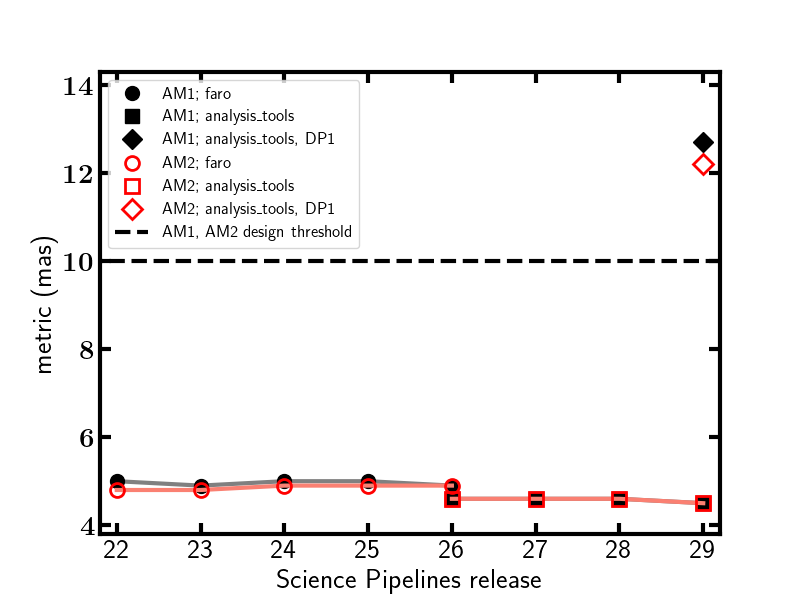
\includegraphics[width=0.475\textwidth, trim=0.0in 0.0in 0.0in 0.0in, clip]{figures/astrom_metrics_v29_with_thresholds.png}
  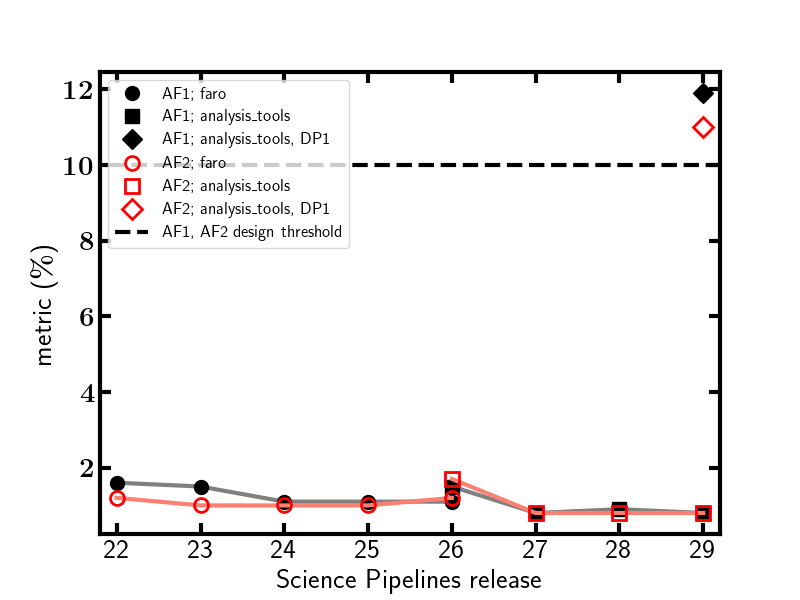
\includegraphics[width=0.475\textwidth, trim=0.0in 0.0in 0.0in 0.0in, clip]{figures/astrom_outlier_metrics_v29_with_thresholds.png}
  \caption{Astrometry metrics measured on $r$-band images compared over the past few major pipelines releases. The figure shows the values of these metrics as measured with \texttt{faro} in versions 22-26 of the LSST Science Pipelines as circles. The measurements from \texttt{analysis\_tools} in versions 26-28 of the Science Pipelines are shown as squares. \textit{Left: } Median astrometric measurement error on 5-arcminute scales (AM1) and 20-arcminute scales (AM2), compared against the SRD requirements (for the ``design'' thresholds; note that the thresholds for AM1 and AM2 are the same, and thus indistinguishable on the figure). \textit{Right: } Fraction of astrometric measurements exceeding the outlier threshold on 5-arcminute (AF1) and 20-arcminute (AF2) scales, compared against the SRD requirements (for the ``design'' thresholds; note that the thresholds for AF1 and AF2 are the same, and thus indistinguishable on the figure). The measured values of the astrometric scatter metrics AM1 and AM2 were virtually unchanged between pipelines version 27 and v28, as were the outlier fractions AF1 and AF2. }
  \label{fig:astrom_metrics}
\end{figure}

The following metrics are defined following LSR-REQ-0094
\citedsp{LSE-29} and Table 18 of \citeds{LPM-17}. Values in this table represent the mean of the results reported by \texttt{analysis\_tools} for the three tracts in RC2.

Any entries left blank are those for which we do not have data in the given filter for that dataset.

\begin{longtable}[]{@{}lllllll@{}}
\toprule
\begin{minipage}[b]{0.12\columnwidth}\raggedright\strut
Metric\strut
\end{minipage} & \begin{minipage}[b]{0.06\columnwidth}\raggedright\strut
Unit\strut
\end{minipage} & \begin{minipage}[b]{0.14\columnwidth}\raggedright\strut
SRD Requirement -- Design\strut
\end{minipage} & \begin{minipage}[b]{0.12\columnwidth}\raggedright\strut
Release 28 Value (RC2) \strut
\end{minipage} & \begin{minipage}[b]{0.12\columnwidth}\raggedright\strut
Release 29 Value (RC2) \strut
\end{minipage} & \begin{minipage}[b]{0.12\columnwidth}\raggedright\strut
Release dp1\_v29 Value (RC2) \strut
\end{minipage} & \begin{minipage}[b]{0.17\columnwidth}\raggedright\strut
Comments\strut
\end{minipage}\tabularnewline
\midrule
\endhead
\begin{minipage}[t]{0.12\columnwidth}\raggedright\strut
AM1: \emph{u}\strut
\end{minipage} & \begin{minipage}[t]{0.06\columnwidth}\raggedright\strut
mas\strut
\end{minipage} & \begin{minipage}[t]{0.14\columnwidth}\raggedright\strut
\(\leq 10.0\)\strut
\end{minipage} & \begin{minipage}[t]{0.12\columnwidth}\raggedright\strut
- \strut
\end{minipage} & \begin{minipage}[t]{0.12\columnwidth}\raggedright\strut
- \strut
\end{minipage} & \begin{minipage}[t]{0.12\columnwidth}\raggedright\strut
18.1 \strut
\end{minipage} & \begin{minipage}[t]{0.17\columnwidth}\raggedright\strut

\end{minipage}\tabularnewline
\begin{minipage}[t]{0.12\columnwidth}\raggedright\strut
AM1: \emph{g}\strut
\end{minipage} & \begin{minipage}[t]{0.06\columnwidth}\raggedright\strut
mas\strut
\end{minipage} & \begin{minipage}[t]{0.14\columnwidth}\raggedright\strut
\(\leq 10.0\)\strut
\end{minipage} & \begin{minipage}[t]{0.12\columnwidth}\raggedright\strut
5.2 \strut
\end{minipage} & \begin{minipage}[t]{0.12\columnwidth}\raggedright\strut
5.0 \strut
\end{minipage} & \begin{minipage}[t]{0.12\columnwidth}\raggedright\strut
15.4 \strut
\end{minipage} & \begin{minipage}[t]{0.17\columnwidth}\raggedright\strut

\end{minipage}\tabularnewline
\begin{minipage}[t]{0.12\columnwidth}\raggedright\strut
AM1: \emph{r}\strut
\end{minipage} & \begin{minipage}[t]{0.06\columnwidth}\raggedright\strut
mas\strut
\end{minipage} & \begin{minipage}[t]{0.14\columnwidth}\raggedright\strut
\(\leq 10.0\)\strut
\end{minipage} & \begin{minipage}[t]{0.12\columnwidth}\raggedright\strut
4.6 \strut
\end{minipage} & \begin{minipage}[t]{0.12\columnwidth}\raggedright\strut
4.5 \strut
\end{minipage} & \begin{minipage}[t]{0.12\columnwidth}\raggedright\strut
12.7 \strut
\end{minipage} & \begin{minipage}[t]{0.17\columnwidth}\raggedright\strut

\end{minipage}\tabularnewline
\begin{minipage}[t]{0.12\columnwidth}\raggedright\strut
AM1: \emph{i}\strut
\end{minipage} & \begin{minipage}[t]{0.06\columnwidth}\raggedright\strut
mas\strut
\end{minipage} & \begin{minipage}[t]{0.14\columnwidth}\raggedright\strut
\(\leq 10.0\)\strut
\end{minipage} & \begin{minipage}[t]{0.12\columnwidth}\raggedright\strut
4.1 \strut
\end{minipage} & \begin{minipage}[t]{0.12\columnwidth}\raggedright\strut
3.9 \strut
\end{minipage} & \begin{minipage}[t]{0.12\columnwidth}\raggedright\strut
11.4 \strut
\end{minipage} & \begin{minipage}[t]{0.17\columnwidth}\raggedright\strut

\end{minipage}\tabularnewline
\begin{minipage}[t]{0.12\columnwidth}\raggedright\strut
AM1: \emph{z}\strut
\end{minipage} & \begin{minipage}[t]{0.06\columnwidth}\raggedright\strut
mas\strut
\end{minipage} & \begin{minipage}[t]{0.14\columnwidth}\raggedright\strut
\(\leq 10.0\)\strut
\end{minipage} & \begin{minipage}[t]{0.12\columnwidth}\raggedright\strut
5.1 \strut
\end{minipage} & \begin{minipage}[t]{0.12\columnwidth}\raggedright\strut
5.0 \strut
\end{minipage} & \begin{minipage}[t]{0.12\columnwidth}\raggedright\strut
11.4 \strut
\end{minipage} & \begin{minipage}[t]{0.17\columnwidth}\raggedright\strut

\end{minipage}\tabularnewline
\begin{minipage}[t]{0.12\columnwidth}\raggedright\strut
AM1: \emph{y}\strut
\end{minipage} & \begin{minipage}[t]{0.06\columnwidth}\raggedright\strut
mas\strut
\end{minipage} & \begin{minipage}[t]{0.14\columnwidth}\raggedright\strut
\(\leq 10.0\)\strut
\end{minipage} & \begin{minipage}[t]{0.12\columnwidth}\raggedright\strut
6.9 \strut
\end{minipage} & \begin{minipage}[t]{0.12\columnwidth}\raggedright\strut
6.8 \strut
\end{minipage} & \begin{minipage}[t]{0.12\columnwidth}\raggedright\strut
12.4 \strut
\end{minipage} & \begin{minipage}[t]{0.17\columnwidth}\raggedright\strut

\end{minipage}\tabularnewline
\begin{minipage}[t]{0.12\columnwidth}\raggedright\strut
AF1: \emph{u}\strut
\end{minipage} & \begin{minipage}[t]{0.06\columnwidth}\raggedright\strut
\%\strut
\end{minipage} & \begin{minipage}[t]{0.14\columnwidth}\raggedright\strut
\(\leq 10.0\)\strut
\end{minipage} & \begin{minipage}[t]{0.12\columnwidth}\raggedright\strut
- \strut
\end{minipage} & \begin{minipage}[t]{0.12\columnwidth}\raggedright\strut
- \strut
\end{minipage} & \begin{minipage}[t]{0.12\columnwidth}\raggedright\strut
24.7 \strut
\end{minipage} & \begin{minipage}[t]{0.17\columnwidth}\raggedright\strut

\end{minipage}\tabularnewline
\begin{minipage}[t]{0.12\columnwidth}\raggedright\strut
AF1: \emph{g}\strut
\end{minipage} & \begin{minipage}[t]{0.06\columnwidth}\raggedright\strut
\%\strut
\end{minipage} & \begin{minipage}[t]{0.14\columnwidth}\raggedright\strut
\(\leq 10.0\)\strut
\end{minipage} & \begin{minipage}[t]{0.12\columnwidth}\raggedright\strut
0.9 \strut
\end{minipage} & \begin{minipage}[t]{0.12\columnwidth}\raggedright\strut
0.8 \strut
\end{minipage} & \begin{minipage}[t]{0.12\columnwidth}\raggedright\strut
24.1 \strut
\end{minipage} & \begin{minipage}[t]{0.17\columnwidth}\raggedright\strut

\end{minipage}\tabularnewline
\begin{minipage}[t]{0.12\columnwidth}\raggedright\strut
AF1: \emph{r}\strut
\end{minipage} & \begin{minipage}[t]{0.06\columnwidth}\raggedright\strut
\%\strut
\end{minipage} & \begin{minipage}[t]{0.14\columnwidth}\raggedright\strut
\(\leq 10.0\)\strut
\end{minipage} & \begin{minipage}[t]{0.12\columnwidth}\raggedright\strut
0.9 \strut
\end{minipage} & \begin{minipage}[t]{0.12\columnwidth}\raggedright\strut
0.8 \strut
\end{minipage} & \begin{minipage}[t]{0.12\columnwidth}\raggedright\strut
11.9 \strut
\end{minipage} & \begin{minipage}[t]{0.17\columnwidth}\raggedright\strut

\end{minipage}\tabularnewline
\begin{minipage}[t]{0.12\columnwidth}\raggedright\strut
AF1: \emph{i}\strut
\end{minipage} & \begin{minipage}[t]{0.06\columnwidth}\raggedright\strut
\%\strut
\end{minipage} & \begin{minipage}[t]{0.14\columnwidth}\raggedright\strut
\(\leq 10.0\)\strut
\end{minipage} & \begin{minipage}[t]{0.12\columnwidth}\raggedright\strut
0.6 \strut
\end{minipage} & \begin{minipage}[t]{0.12\columnwidth}\raggedright\strut
0.6 \strut
\end{minipage} & \begin{minipage}[t]{0.12\columnwidth}\raggedright\strut
8.7 \strut
\end{minipage} & \begin{minipage}[t]{0.17\columnwidth}\raggedright\strut

\end{minipage}\tabularnewline
\begin{minipage}[t]{0.12\columnwidth}\raggedright\strut
AF1: \emph{z}\strut
\end{minipage} & \begin{minipage}[t]{0.06\columnwidth}\raggedright\strut
\%\strut
\end{minipage} & \begin{minipage}[t]{0.14\columnwidth}\raggedright\strut
\(\leq 10.0\)\strut
\end{minipage} & \begin{minipage}[t]{0.12\columnwidth}\raggedright\strut
0.6 \strut
\end{minipage} & \begin{minipage}[t]{0.12\columnwidth}\raggedright\strut
0.6 \strut
\end{minipage} & \begin{minipage}[t]{0.12\columnwidth}\raggedright\strut
9.6 \strut
\end{minipage} & \begin{minipage}[t]{0.17\columnwidth}\raggedright\strut

\end{minipage}\tabularnewline
\begin{minipage}[t]{0.12\columnwidth}\raggedright\strut
AF1: \emph{y}\strut
\end{minipage} & \begin{minipage}[t]{0.06\columnwidth}\raggedright\strut
\%\strut
\end{minipage} & \begin{minipage}[t]{0.14\columnwidth}\raggedright\strut
\(\leq 10.0\)\strut
\end{minipage} & \begin{minipage}[t]{0.12\columnwidth}\raggedright\strut
2.9 \strut
\end{minipage} & \begin{minipage}[t]{0.12\columnwidth}\raggedright\strut
2.8 \strut
\end{minipage} & \begin{minipage}[t]{0.12\columnwidth}\raggedright\strut
12.0 \strut
\end{minipage} & \begin{minipage}[t]{0.17\columnwidth}\raggedright\strut

\end{minipage}\tabularnewline
\begin{minipage}[t]{0.12\columnwidth}\raggedright\strut
AD1: \emph{u}\strut
\end{minipage} & \begin{minipage}[t]{0.06\columnwidth}\raggedright\strut
mas\strut
\end{minipage} & \begin{minipage}[t]{0.14\columnwidth}\raggedright\strut
\(\leq 20.0\)\strut
\end{minipage} & \begin{minipage}[t]{0.12\columnwidth}\raggedright\strut
- \strut
\end{minipage} & \begin{minipage}[t]{0.12\columnwidth}\raggedright\strut
- \strut
\end{minipage} & \begin{minipage}[t]{0.12\columnwidth}\raggedright\strut
30.4 \strut
\end{minipage} & \begin{minipage}[t]{0.17\columnwidth}\raggedright\strut

\end{minipage}\tabularnewline
\begin{minipage}[t]{0.12\columnwidth}\raggedright\strut
AD1: \emph{g}\strut
\end{minipage} & \begin{minipage}[t]{0.06\columnwidth}\raggedright\strut
mas\strut
\end{minipage} & \begin{minipage}[t]{0.14\columnwidth}\raggedright\strut
\(\leq 20.0\)\strut
\end{minipage} & \begin{minipage}[t]{0.12\columnwidth}\raggedright\strut
9.7 \strut
\end{minipage} & \begin{minipage}[t]{0.12\columnwidth}\raggedright\strut
9.6 \strut
\end{minipage} & \begin{minipage}[t]{0.12\columnwidth}\raggedright\strut
30.8 \strut
\end{minipage} & \begin{minipage}[t]{0.17\columnwidth}\raggedright\strut

\end{minipage}\tabularnewline
\begin{minipage}[t]{0.12\columnwidth}\raggedright\strut
AD1: \emph{r}\strut
\end{minipage} & \begin{minipage}[t]{0.06\columnwidth}\raggedright\strut
mas\strut
\end{minipage} & \begin{minipage}[t]{0.14\columnwidth}\raggedright\strut
\(\leq 20.0\)\strut
\end{minipage} & \begin{minipage}[t]{0.12\columnwidth}\raggedright\strut
9.2 \strut
\end{minipage} & \begin{minipage}[t]{0.12\columnwidth}\raggedright\strut
9.0 \strut
\end{minipage} & \begin{minipage}[t]{0.12\columnwidth}\raggedright\strut
21.3 \strut
\end{minipage} & \begin{minipage}[t]{0.17\columnwidth}\raggedright\strut

\end{minipage}\tabularnewline
\begin{minipage}[t]{0.12\columnwidth}\raggedright\strut
AD1: \emph{i}\strut
\end{minipage} & \begin{minipage}[t]{0.06\columnwidth}\raggedright\strut
mas\strut
\end{minipage} & \begin{minipage}[t]{0.14\columnwidth}\raggedright\strut
\(\leq 20.0\)\strut
\end{minipage} & \begin{minipage}[t]{0.12\columnwidth}\raggedright\strut
7.9 \strut
\end{minipage} & \begin{minipage}[t]{0.12\columnwidth}\raggedright\strut
7.7 \strut
\end{minipage} & \begin{minipage}[t]{0.12\columnwidth}\raggedright\strut
19.1 \strut
\end{minipage} & \begin{minipage}[t]{0.17\columnwidth}\raggedright\strut

\end{minipage}\tabularnewline
\begin{minipage}[t]{0.12\columnwidth}\raggedright\strut
AD1: \emph{z}\strut
\end{minipage} & \begin{minipage}[t]{0.06\columnwidth}\raggedright\strut
mas\strut
\end{minipage} & \begin{minipage}[t]{0.14\columnwidth}\raggedright\strut
\(\leq 20.0\)\strut
\end{minipage} & \begin{minipage}[t]{0.12\columnwidth}\raggedright\strut
9.6 \strut
\end{minipage} & \begin{minipage}[t]{0.12\columnwidth}\raggedright\strut
9.6 \strut
\end{minipage} & \begin{minipage}[t]{0.12\columnwidth}\raggedright\strut
19.7 \strut
\end{minipage} & \begin{minipage}[t]{0.17\columnwidth}\raggedright\strut

\end{minipage}\tabularnewline
\begin{minipage}[t]{0.12\columnwidth}\raggedright\strut
AD1: \emph{y}\strut
\end{minipage} & \begin{minipage}[t]{0.06\columnwidth}\raggedright\strut
mas\strut
\end{minipage} & \begin{minipage}[t]{0.14\columnwidth}\raggedright\strut
\(\leq 20.0\)\strut
\end{minipage} & \begin{minipage}[t]{0.12\columnwidth}\raggedright\strut
12.6 \strut
\end{minipage} & \begin{minipage}[t]{0.12\columnwidth}\raggedright\strut
12.5 \strut
\end{minipage} & \begin{minipage}[t]{0.12\columnwidth}\raggedright\strut
21.4 \strut
\end{minipage} & \begin{minipage}[t]{0.17\columnwidth}\raggedright\strut

\end{minipage}\tabularnewline
\begin{minipage}[t]{0.12\columnwidth}\raggedright\strut
AM2: \emph{u}\strut
\end{minipage} & \begin{minipage}[t]{0.06\columnwidth}\raggedright\strut
mas\strut
\end{minipage} & \begin{minipage}[t]{0.14\columnwidth}\raggedright\strut
\(\leq 10.0\)\strut
\end{minipage} & \begin{minipage}[t]{0.12\columnwidth}\raggedright\strut
- \strut
\end{minipage} & \begin{minipage}[t]{0.12\columnwidth}\raggedright\strut
- \strut
\end{minipage} & \begin{minipage}[t]{0.12\columnwidth}\raggedright\strut
17.0 \strut
\end{minipage} & \begin{minipage}[t]{0.17\columnwidth}\raggedright\strut

\end{minipage}\tabularnewline
\begin{minipage}[t]{0.12\columnwidth}\raggedright\strut
AM2: \emph{g}\strut
\end{minipage} & \begin{minipage}[t]{0.06\columnwidth}\raggedright\strut
mas\strut
\end{minipage} & \begin{minipage}[t]{0.14\columnwidth}\raggedright\strut
\(\leq 10.0\)\strut
\end{minipage} & \begin{minipage}[t]{0.12\columnwidth}\raggedright\strut
5.3 \strut
\end{minipage} & \begin{minipage}[t]{0.12\columnwidth}\raggedright\strut
5.2 \strut
\end{minipage} & \begin{minipage}[t]{0.12\columnwidth}\raggedright\strut
15.4 \strut
\end{minipage} & \begin{minipage}[t]{0.17\columnwidth}\raggedright\strut

\end{minipage}\tabularnewline
\begin{minipage}[t]{0.12\columnwidth}\raggedright\strut
AM2: \emph{r}\strut
\end{minipage} & \begin{minipage}[t]{0.06\columnwidth}\raggedright\strut
mas\strut
\end{minipage} & \begin{minipage}[t]{0.14\columnwidth}\raggedright\strut
\(\leq 10.0\)\strut
\end{minipage} & \begin{minipage}[t]{0.12\columnwidth}\raggedright\strut
4.6 \strut
\end{minipage} & \begin{minipage}[t]{0.12\columnwidth}\raggedright\strut
4.5 \strut
\end{minipage} & \begin{minipage}[t]{0.12\columnwidth}\raggedright\strut
12.2 \strut
\end{minipage} & \begin{minipage}[t]{0.17\columnwidth}\raggedright\strut

\end{minipage}\tabularnewline
\begin{minipage}[t]{0.12\columnwidth}\raggedright\strut
AM2: \emph{i}\strut
\end{minipage} & \begin{minipage}[t]{0.06\columnwidth}\raggedright\strut
mas\strut
\end{minipage} & \begin{minipage}[t]{0.14\columnwidth}\raggedright\strut
\(\leq 10.0\)\strut
\end{minipage} & \begin{minipage}[t]{0.12\columnwidth}\raggedright\strut
4.0 \strut
\end{minipage} & \begin{minipage}[t]{0.12\columnwidth}\raggedright\strut
3.9 \strut
\end{minipage} & \begin{minipage}[t]{0.12\columnwidth}\raggedright\strut
11.0 \strut
\end{minipage} & \begin{minipage}[t]{0.17\columnwidth}\raggedright\strut

\end{minipage}\tabularnewline
\begin{minipage}[t]{0.12\columnwidth}\raggedright\strut
AM2: \emph{z}\strut
\end{minipage} & \begin{minipage}[t]{0.06\columnwidth}\raggedright\strut
mas\strut
\end{minipage} & \begin{minipage}[t]{0.14\columnwidth}\raggedright\strut
\(\leq 10.0\)\strut
\end{minipage} & \begin{minipage}[t]{0.12\columnwidth}\raggedright\strut
5.2 \strut
\end{minipage} & \begin{minipage}[t]{0.12\columnwidth}\raggedright\strut
5.1 \strut
\end{minipage} & \begin{minipage}[t]{0.12\columnwidth}\raggedright\strut
10.8 \strut
\end{minipage} & \begin{minipage}[t]{0.17\columnwidth}\raggedright\strut

\end{minipage}\tabularnewline
\begin{minipage}[t]{0.12\columnwidth}\raggedright\strut
AM2: \emph{y}\strut
\end{minipage} & \begin{minipage}[t]{0.06\columnwidth}\raggedright\strut
mas\strut
\end{minipage} & \begin{minipage}[t]{0.14\columnwidth}\raggedright\strut
\(\leq 10.0\)\strut
\end{minipage} & \begin{minipage}[t]{0.12\columnwidth}\raggedright\strut
7.1 \strut
\end{minipage} & \begin{minipage}[t]{0.12\columnwidth}\raggedright\strut
6.9 \strut
\end{minipage} & \begin{minipage}[t]{0.12\columnwidth}\raggedright\strut
11.6 \strut
\end{minipage} & \begin{minipage}[t]{0.17\columnwidth}\raggedright\strut

\end{minipage}\tabularnewline
\begin{minipage}[t]{0.12\columnwidth}\raggedright\strut
AF2: \emph{u}\strut
\end{minipage} & \begin{minipage}[t]{0.06\columnwidth}\raggedright\strut
\%\strut
\end{minipage} & \begin{minipage}[t]{0.14\columnwidth}\raggedright\strut
\(\leq 10.0\)\strut
\end{minipage} & \begin{minipage}[t]{0.12\columnwidth}\raggedright\strut
- \strut
\end{minipage} & \begin{minipage}[t]{0.12\columnwidth}\raggedright\strut
- \strut
\end{minipage} & \begin{minipage}[t]{0.12\columnwidth}\raggedright\strut
24.1 \strut
\end{minipage} & \begin{minipage}[t]{0.17\columnwidth}\raggedright\strut

\end{minipage}\tabularnewline
\begin{minipage}[t]{0.12\columnwidth}\raggedright\strut
AF2: \emph{g}\strut
\end{minipage} & \begin{minipage}[t]{0.06\columnwidth}\raggedright\strut
\%\strut
\end{minipage} & \begin{minipage}[t]{0.14\columnwidth}\raggedright\strut
\(\leq 10.0\)\strut
\end{minipage} & \begin{minipage}[t]{0.12\columnwidth}\raggedright\strut
0.9 \strut
\end{minipage} & \begin{minipage}[t]{0.12\columnwidth}\raggedright\strut
0.9 \strut
\end{minipage} & \begin{minipage}[t]{0.12\columnwidth}\raggedright\strut
24.7 \strut
\end{minipage} & \begin{minipage}[t]{0.17\columnwidth}\raggedright\strut

\end{minipage}\tabularnewline
\begin{minipage}[t]{0.12\columnwidth}\raggedright\strut
AF2: \emph{r}\strut
\end{minipage} & \begin{minipage}[t]{0.06\columnwidth}\raggedright\strut
\%\strut
\end{minipage} & \begin{minipage}[t]{0.14\columnwidth}\raggedright\strut
\(\leq 10.0\)\strut
\end{minipage} & \begin{minipage}[t]{0.12\columnwidth}\raggedright\strut
0.8 \strut
\end{minipage} & \begin{minipage}[t]{0.12\columnwidth}\raggedright\strut
0.8 \strut
\end{minipage} & \begin{minipage}[t]{0.12\columnwidth}\raggedright\strut
11.0 \strut
\end{minipage} & \begin{minipage}[t]{0.17\columnwidth}\raggedright\strut

\end{minipage}\tabularnewline
\begin{minipage}[t]{0.12\columnwidth}\raggedright\strut
AF2: \emph{i}\strut
\end{minipage} & \begin{minipage}[t]{0.06\columnwidth}\raggedright\strut
\%\strut
\end{minipage} & \begin{minipage}[t]{0.14\columnwidth}\raggedright\strut
\(\leq 10.0\)\strut
\end{minipage} & \begin{minipage}[t]{0.12\columnwidth}\raggedright\strut
0.6 \strut
\end{minipage} & \begin{minipage}[t]{0.12\columnwidth}\raggedright\strut
0.5 \strut
\end{minipage} & \begin{minipage}[t]{0.12\columnwidth}\raggedright\strut
8.1 \strut
\end{minipage} & \begin{minipage}[t]{0.17\columnwidth}\raggedright\strut

\end{minipage}\tabularnewline
\begin{minipage}[t]{0.12\columnwidth}\raggedright\strut
AF2: \emph{z}\strut
\end{minipage} & \begin{minipage}[t]{0.06\columnwidth}\raggedright\strut
\%\strut
\end{minipage} & \begin{minipage}[t]{0.14\columnwidth}\raggedright\strut
\(\leq 10.0\)\strut
\end{minipage} & \begin{minipage}[t]{0.12\columnwidth}\raggedright\strut
0.7 \strut
\end{minipage} & \begin{minipage}[t]{0.12\columnwidth}\raggedright\strut
0.7 \strut
\end{minipage} & \begin{minipage}[t]{0.12\columnwidth}\raggedright\strut
8.4 \strut
\end{minipage} & \begin{minipage}[t]{0.17\columnwidth}\raggedright\strut

\end{minipage}\tabularnewline
\begin{minipage}[t]{0.12\columnwidth}\raggedright\strut
AF2: \emph{y}\strut
\end{minipage} & \begin{minipage}[t]{0.06\columnwidth}\raggedright\strut
\%\strut
\end{minipage} & \begin{minipage}[t]{0.14\columnwidth}\raggedright\strut
\(\leq 10.0\)\strut
\end{minipage} & \begin{minipage}[t]{0.12\columnwidth}\raggedright\strut
3.2 \strut
\end{minipage} & \begin{minipage}[t]{0.12\columnwidth}\raggedright\strut
3.2 \strut
\end{minipage} & \begin{minipage}[t]{0.12\columnwidth}\raggedright\strut
10.7 \strut
\end{minipage} & \begin{minipage}[t]{0.17\columnwidth}\raggedright\strut

\end{minipage}\tabularnewline
\begin{minipage}[t]{0.12\columnwidth}\raggedright\strut
AD2: \emph{u}\strut
\end{minipage} & \begin{minipage}[t]{0.06\columnwidth}\raggedright\strut
mas\strut
\end{minipage} & \begin{minipage}[t]{0.14\columnwidth}\raggedright\strut
\(\leq 20.0\)\strut
\end{minipage} & \begin{minipage}[t]{0.12\columnwidth}\raggedright\strut
- \strut
\end{minipage} & \begin{minipage}[t]{0.12\columnwidth}\raggedright\strut
- \strut
\end{minipage} & \begin{minipage}[t]{0.12\columnwidth}\raggedright\strut
30.0 \strut
\end{minipage} & \begin{minipage}[t]{0.17\columnwidth}\raggedright\strut

\end{minipage}\tabularnewline
\begin{minipage}[t]{0.12\columnwidth}\raggedright\strut
AD2: \emph{g}\strut
\end{minipage} & \begin{minipage}[t]{0.06\columnwidth}\raggedright\strut
mas\strut
\end{minipage} & \begin{minipage}[t]{0.14\columnwidth}\raggedright\strut
\(\leq 20.0\)\strut
\end{minipage} & \begin{minipage}[t]{0.12\columnwidth}\raggedright\strut
10.0 \strut
\end{minipage} & \begin{minipage}[t]{0.12\columnwidth}\raggedright\strut
9.8 \strut
\end{minipage} & \begin{minipage}[t]{0.12\columnwidth}\raggedright\strut
31.5 \strut
\end{minipage} & \begin{minipage}[t]{0.17\columnwidth}\raggedright\strut

\end{minipage}\tabularnewline
\begin{minipage}[t]{0.12\columnwidth}\raggedright\strut
AD2: \emph{r}\strut
\end{minipage} & \begin{minipage}[t]{0.06\columnwidth}\raggedright\strut
mas\strut
\end{minipage} & \begin{minipage}[t]{0.14\columnwidth}\raggedright\strut
\(\leq 20.0\)\strut
\end{minipage} & \begin{minipage}[t]{0.12\columnwidth}\raggedright\strut
9.3 \strut
\end{minipage} & \begin{minipage}[t]{0.12\columnwidth}\raggedright\strut
9.2 \strut
\end{minipage} & \begin{minipage}[t]{0.12\columnwidth}\raggedright\strut
20.7 \strut
\end{minipage} & \begin{minipage}[t]{0.17\columnwidth}\raggedright\strut

\end{minipage}\tabularnewline
\begin{minipage}[t]{0.12\columnwidth}\raggedright\strut
AD2: \emph{i}\strut
\end{minipage} & \begin{minipage}[t]{0.06\columnwidth}\raggedright\strut
mas\strut
\end{minipage} & \begin{minipage}[t]{0.14\columnwidth}\raggedright\strut
\(\leq 20.0\)\strut
\end{minipage} & \begin{minipage}[t]{0.12\columnwidth}\raggedright\strut
7.9 \strut
\end{minipage} & \begin{minipage}[t]{0.12\columnwidth}\raggedright\strut
7.6 \strut
\end{minipage} & \begin{minipage}[t]{0.12\columnwidth}\raggedright\strut
18.6 \strut
\end{minipage} & \begin{minipage}[t]{0.17\columnwidth}\raggedright\strut

\end{minipage}\tabularnewline
\begin{minipage}[t]{0.12\columnwidth}\raggedright\strut
AD2: \emph{z}\strut
\end{minipage} & \begin{minipage}[t]{0.06\columnwidth}\raggedright\strut
mas\strut
\end{minipage} & \begin{minipage}[t]{0.14\columnwidth}\raggedright\strut
\(\leq 20.0\)\strut
\end{minipage} & \begin{minipage}[t]{0.12\columnwidth}\raggedright\strut
9.9 \strut
\end{minipage} & \begin{minipage}[t]{0.12\columnwidth}\raggedright\strut
9.8 \strut
\end{minipage} & \begin{minipage}[t]{0.12\columnwidth}\raggedright\strut
18.8 \strut
\end{minipage} & \begin{minipage}[t]{0.17\columnwidth}\raggedright\strut

\end{minipage}\tabularnewline
\begin{minipage}[t]{0.12\columnwidth}\raggedright\strut
AD2: \emph{y}\strut
\end{minipage} & \begin{minipage}[t]{0.06\columnwidth}\raggedright\strut
mas\strut
\end{minipage} & \begin{minipage}[t]{0.14\columnwidth}\raggedright\strut
\(\leq 20.0\)\strut
\end{minipage} & \begin{minipage}[t]{0.12\columnwidth}\raggedright\strut
12.9 \strut
\end{minipage} & \begin{minipage}[t]{0.12\columnwidth}\raggedright\strut
12.8 \strut
\end{minipage} & \begin{minipage}[t]{0.12\columnwidth}\raggedright\strut
20.4 \strut
\end{minipage} & \begin{minipage}[t]{0.17\columnwidth}\raggedright\strut

\end{minipage}\tabularnewline
\bottomrule
\end{longtable}

\appendix

% Include all the relevant bib files.
% https://lsst-texmf.lsst.io/lsstdoc.html#bibliographies
\section{References} \label{sec:bib}
\renewcommand{\refname}{} % Suppress default Bibliography section
\bibliography{local,lsst,lsst-dm,refs_ads,refs,books}

% Make sure lsst-texmf/bin/generateAcronyms.py is in your path
\section{Acronyms} \label{sec:acronyms}
\input{acronyms.tex}
% If you want glossary uncomment below and comment out the two lines above.
% \printglossaries

\end{document}
